% -*- mode: LaTeX; TeX-PDF-mode: t; -*-
\input{./econtexRoot}\documentclass[\econtexRoot/ProjectMMD]{subfiles}
\input{./econtexRoot}\input{\LaTeXInputs/econtex_onlyinsubfile}
\onlyinsubfile{\externaldocument{\LaTeXGenerated/ProjectMMD}} % Get xrefs -- esp to appendix -- from main file; only works properly if main file has already been compiled;

\begin{document}
\section{Rectifying the solution to this model with Bover's solution}

\cite{bover1991relaxing} did not take the same solution approach as this paper. In the original, Bover solves the intertemporal problem with a Lagrangian and a clever transformation of the budget constraint. Yet, my approach using a Bellman equation produces a sligtly different looking solution. Yet, the two are indeed the same. Bover's solution regarding consumption takes the following form:

\begin{align*}
  c_t &= \gamma_c + B_2 \lambda_t^{-1}
\end{align*}

To see that my solution is the same, we first look at the consumption Euler equation I derived earlier. This provides a very clear relationship between $c_t -\gamma_c$  and $c_{t+1} -\gamma_c$.
\begin{align*}
\frac{c_t - \gamma_c}{c_{t+1} - \gamma_c} &= \frac{1+\rho}{1+r}
\end{align*}

According to the solution in \cite{bover1991relaxing}, we can use Equation 7 in her paper to obtain a similar ratio.
\begin{align*}
  \frac{c_t - \gamma_c}{c_{t+1}-\gamma_c} &=  \frac{\lambda_t^{-1}}{\lambda_{t+1}^{-1}}
\end{align*}

Therefore, a simple test will be to see if the ratio of the inverse lagrange multipliers is equal to $(1+\rho) / (1+r)$. The code is created using the Bover notation, which allows us to see if there are any bugs in the code.

\begin{figure}[ht]
  \centerline{
    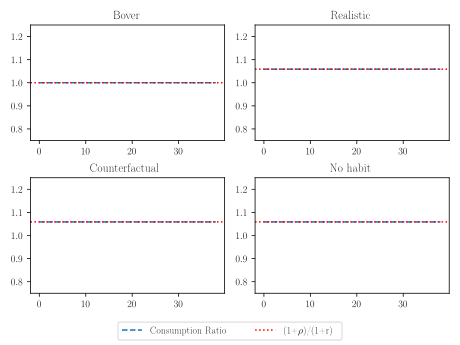
\includegraphics[width=6.0in]{\FigDir/inter_consumption.png}
  }
  \caption{Consumption between time $t$ and $t+1$} \label{fig:inter_consumption}
%\centerline{See Table~\ref{table:Calibration} for Numerical Values of Nodes Under Baseline Parameters}
\end{figure}


Figure \ref{fig:inter_consumption} demonstrates that we do indeed observe a constant relationship between $c_t -\gamma_c$ and $c_{t+1} - \gamma_c$. Thus, we conclude that the ratio of subsequent Lagrange multipliers is $(1+\rho)/(1+r)$.


Bover solves this problem in terms of labor hours, but this does not prove any difficulty since our time constraint will tell us that $l_t = T-h_t$. Thus, Bover's equation 6 suggests that the ratio of leisure hours will be:
\begin{align}
  \frac{ l_t - \varphi l_{t-1} - \gamma_l}{l_{t+1} - \varphi l_t - \gamma_l} &= \frac{\lambda_t^{-1}}{\lambda_{t+1}^{-1}} \frac{w_{t+1}^{+}}{w_t^{+}} \label{eq:bover_focl}
\end{align}
where
\begin{align*}
  w_k^{+} &=W \sum_{j=0}^{T-k}\left( \frac{\varphi}{1+r}\right) ^j
\end{align*}

The hope is that starting from our FOC for leisure and using the Bover's FOC for hours (leisure), we hope to arrive at some tautology. For notational simplicity, let $\hat{l}_i =l_i - \varphi l_{i-1} - \gamma_l$. Starting from our FOC for leisure:
\begin{align*}
  \frac{B_1}{\hat{l}_t} &= \frac{B_2 W}{c_t - \gamma_c} + \frac{B_1\frac{ \varphi}{1+\rho}}{\hat{l}_{t+1}} \\
  \frac{w_t^{+}}{\lambda_t^{-1}} &= \frac{W}{\lambda_t^{-1}} + \frac{w_{t+1}^{+} \frac{\varphi}{1+rho}}{\lambda_{t+1}^{-1}} \\
  \frac{1 - \left( \frac{\varphi}{1+r} \right)^{T-t+1}}{1- \frac{\varphi}{1+r}} &= 1 + \frac{\varphi}{1+\rho}\cdot \frac{1+\rho}{1+r} \frac{1 - \left( \frac{\varphi}{1+r} \right)^{T-t}}{1- \frac{\varphi}{1+r}}  \\
  1 - \left( \frac{\varphi}{1+r} \right)^{T-t+1} &=\left(1 - \frac{\varphi}{1+r}\right) +\frac{\varphi}{1+r} \left( 1- \left( \frac{\varphi}{1+r}\right)^{T-t} \right) \\
  1 - \left( \frac{\varphi}{1+r} \right)^{T-t+1} &= 1 - \left( \frac{\varphi}{1+r} \right)^{T-t+1}
\end{align*}
This tautology suggests that both approaches yield the same solution.

%\bibliography{\econtexRoot/\texname,\econtexBib}
\onlyinsubfile{\input{\LaTeXInputs/bibliography_blend}}

\end{document}

% Local Variables:
% eval: (setq TeX-command-list  (assq-delete-all (car (assoc "BibTeX" TeX-command-list)) TeX-command-list))
% eval: (setq TeX-command-list  (assq-delete-all (car (assoc "BibTeX" TeX-command-list)) TeX-command-list))
% eval: (setq TeX-command-list  (assq-delete-all (car (assoc "Biber"  TeX-command-list)) TeX-command-list))
% eval: (setq TeX-command-list  (remove '("BibTeX" "%(bibtex) LaTeX/%s"    TeX-run-BibTeX nil t :help "Run BibTeX") TeX-command-list))
% eval: (setq TeX-command-list  (remove '("BibTeX" "bibtex LaTeX/%s"    TeX-run-BibTeX nil t :help "Run BibTeX") TeX-command-list))
% eval: (add-to-list 'TeX-command-list '("BibTeX" "bibtex ../LaTeX/%s" TeX-run-BibTeX nil t                                                                              :help "Run BibTeX") t)
% eval: (add-to-list 'TeX-command-list '("BibTeX" "bibtex ../LaTeX/%s" TeX-run-BibTeX nil (plain-tex-mode latex-mode doctex-mode ams-tex-mode texinfo-mode context-mode) :help "Run BibTeX") t)
% TeX-PDF-mode: t
% TeX-file-line-error: t
% TeX-debug-warnings: t
% TeX-source-correlate-mode: t
% TeX-parse-self: t
% LaTeX-command-style: (("" "%(PDF)%(latex) %(file-line-error) %(extraopts) -output-directory=../LaTeX %S%(PDFout)"))
% eval: (cond ((string-equal system-type "darwin") (progn (setq TeX-view-program-list '(("Skim" "/Applications/Skim.app/Contents/SharedSupport/displayline -b %n ../LaTeX/%o %b"))))))
% eval: (cond ((string-equal system-type "gnu/linux") (progn (setq TeX-view-program-list '(("Evince" "evince --page-index=%(outpage) ../LaTeX/%o"))))))
% eval: (cond ((string-equal system-type "gnu/linux") (progn (setq TeX-view-program-selection '((output-pdf "Evince"))))))
% TeX-parse-all-errors: t
% End:
